%=====================
\chapter{Requirements}
%=====================
\label{chap:req:requirements}
This chapter describes an utility that creates Wireshark dissectors from C
header files. The dissectors must interpret binary representations of C
structs. In \autoref{sec:req:list} we give a high level overview of the
utility and lists all the functional and non-function requirements.

\hyperref[sec:req:stories]{Section \ref*{sec:req:stories}} gives user stories
for the requirements, while \autoref{sec:req:usecases} provides use cases for
the utility, and \autoref{sec:prodbacklog} contains the complete product
backlog.

%-----------------------------
\section{List of requirements}
%-----------------------------
\label{sec:req:list}

\subsection{Overview}
%-----------------
We are to create an utility that allows Wireshark to interpret the binary
representations of C-language structs. While C structs seldom are exchanged
across networks, they are sometimes used in inter-process communication. The
purpose of the utility described here is to provide Wireshark with the
capability of automatically dissecting the binary representation of a C struct,
as long as its definition is known.

The expected work flow for the utility is to read one or more C header files,
which contain struct definitions, and output Wireshark dissectors, implemented
in Lua scripts. A configuration file or source code annotations in the header
files may be used when additional configuration is required.

\autoref{tab:req:func} lists the functional requirements, while
\autoref{tab:req:nonfunc} lists the non-functional requirements. Each
requirement have a priority (Pri) and a complexity (Cmp): High (H), 
Medium (M) or Low (L) which is explained in \autoref{sec:req:priority} and
\autoref{sec:req:compl}.

\subsection{Prioritization}
%--------------------------
\label{sec:req:priority}
The team has, in cooperation with the customer, prioritized the requirements
in three categories:
\begin{inparaenum}[\itshape a\upshape)]
	\item High,
	\item Medium or
	\item Low.
\end{inparaenum} 

\begin{description}
	\item[High] Core functionality of the utility which must be implemented.
	\item[Medium] Requirements that will improve the value of the utility.
	\item[Low] Requirements that will not add much value to the utility.
\end{description}

\subsection{Complexity}
%----------------------
\label{sec:req:compl}
The team has estimated the complexity for each requirement. We use the same
categories as for requirements priority:
\begin{inparaenum}[\itshape a\upshape)]
	\item High,
	\item Medium or
	\item Low.
\end{inparaenum} 

\begin{description}
	\item[High] Functionality which seems difficult and non-trivial to create.
	\item[Medium] Functionality that seems time consuming but straight forward.
	\item[Low] Requirements that are trivial to implement.
\end{description}

%%%%%%%%%%%%%%%%%%%%%%%%%%%%%%%%%%%%
%%%%%%%%%%%%%%%%%%%%%%%%%%%%%%%%%%%%
%        OBS OBS OBS OBS
%
% These requirements are duplicated
% in many different locations,
% remember to update them all
%
% * product backlog
% * user stories
% * sprint 1 backlog
% * anywhere else?
%
%%%%%%%%%%%%%%%%%%%%%%%%%%%%%%%%%%%%
%%%%%%%%%%%%%%%%%%%%%%%%%%%%%%%%%%%%
\begin{table}[htbp] \footnotesize \center
\caption{Functional Requirements\label{tab:req:func}}
\noindent\makebox[\textwidth]{%
\begin{tabularx}{1.2\textwidth}{l X c c}
	\toprule
	ID & Description & Pri. & Cmp. \\
	\midrule
	FR1 & The utility must be able to read basic C language struct definitions from C header files & H & \\
	FR1-A & The utility must support the following basic data types: int, float, char and boolean & H & L \\
	FR1-B & The utility must support members of type enum & H & L \\
	FR1-C & The utility must support members of type struct & H & M \\
	FR1-D & The utility must support members of type union & M & M \\
	FR1-E & The utility must support members of type array & H & M \\
	FR1-F & The utility should detect structs with the same name, and report it as an error & M & L \\
	\midrule
	FR2 & The utility must be able to generate Lua dissectors for Wireshark for the binary representation of C struct & H & \\
	FR2-A & The dissector shall be able to display simple structs & H & L \\
	FR2-B & The dissector shall be able to support structs within structs & M & M \\
	FR2-C & The dissector must support Wireshark's built-in filter and search on attributes & H & L \\
	FR2-D & The dissector shall be able to recognize invalid values for a struct member & L & L \\
	\midrule
	FR3 & The utility must support C preprocessor directives and macros & H & \\
	FR3-A & The utility shall support \#include & H & L \\
	FR3-B & The utility shall support \#define and \#if & H & L \\
	FR3-C & The utility shall support \verb+WIN32+, \verb+_WIN32+, \verb+_WIN64+, \verb+__sparc__+, \verb+__sparc+ and \verb+sun+ & M & H \\
	\midrule
	FR4 & The utility must support user configuration & M & \\
	FR4-A & Configuration must support valid ranges for struct members & L & L \\
	FR4-B & Configuration must support custom Lua files for specific protocols & H & H \\
	FR4-C & Configuration must support custom handling of specific data types & L & M \\
	FR4-D & Configuration must support specifying the ID of dissectors & H & L \\
	FR4-E & Configuration must support various trailers (other registered protocol) & L & H \\
	FR4-F & Configuration must support integer members which represent enumerated named value & M & L \\	
	FR4-G & Configuration must support members which are bit string & M & L \\
	\midrule
	FR5 & The dissectors must be able to handle binary input which size and endian depends on originating platform & M & \\
	FR5-A & Flags must be specified in configuration for each platform & M & M \\
	FR5-B & Generate dissectors with correct alignment depending on platform & M & M \\
	FR5-C & Generate dissectors which support both little and big endian platforms & H & M \\
	FR5-D & Generate dissectors which support different sizes depending on platforms & M & H \\
	\midrule
	FR6 & The utility shall support parameters from command line & H & \\
	FR6-A & Command line shall support parameter for C header file & H & L \\
	FR6-B & Command line shall support parameter for configuration file & H & L \\
	FR6-C & Command line shall support batch processing of C header and configuration files & L & M \\
	FR6-D & When running batch mode, dissectors that already are generated, shall not be regenerated, if the source are not modified since last run & L & M \\
	\bottomrule
\end{tabularx}}
\end{table}

\begin{table}[htbp] \footnotesize \center
\caption{Non-Functional Requirements\label{tab:req:nonfunc}}
\noindent\makebox[\textwidth]{%
\begin{tabularx}{1.2\textwidth}{l X c c}
	\toprule
	ID & Description & Pri. & Cmp. \\
	\midrule
	NR1 & The utility shall be able to run on latest Windows and Solaris operating system & M & L \\
	\addlinespace
	NR2 & The dissector shall be able to run on Windows x86, Windows x86-64, Solaris x86, Solaris x86-64 and Solaris SPARC & M & M \\
	\addlinespace
	NR3 & The utility shall only have a command line user interface. No GUI \& clicking! & H & L \\
	\addlinespace
	NR4 & The utility must have sufficient documentation to allow a person, with no previous knowledge of the system or Wireshark, to be able to use it to generate Lua dissectors after 5 hours of reading & M & M \\
	\addlinespace
	NR5 & The utility must have sufficient documentation to allow a person, already proficient with the system, to be able to extend its functionality after Y hours of reading & M & M \\
	\addlinespace
	NR6 & The utility code should follow standard python coding convention as specified by PEP8 and try to follow python style guidelines defined by PEP20 & H & L \\
	\addlinespace
	NR7 & All Python modules, classes, functions and methods in the utility should have docstrings which explains their code & L & L \\
	\bottomrule
\end{tabularx}}
\end{table}


%---------------------
\section{User Stories}
%---------------------
\label{sec:req:stories}
\subsection{Sprint 1}
\label{sec:req:stories1}
This section lists the user stories for the first sprint, these are displayed in \autoref{tab:req:stories1} and \autoref{tab:req:stories2}.
As we are developing a very technical utility we have written user stories with an implementation level of abstraction. 
These user stories represent how we intend to add the functionality of the each requirement to the utility.
The administrator in this context is the administrator at Thales Norway AS. 
The developer is the person that uses Wireshark with the dissector generated by CSjark.
This section is subject to change throughout the sprint, as we do not know all the details yet.


\begin{table}[htbp] \footnotesize \center
\caption{User stories - Sprint 1 part 1\label{tab:req:stories1}}
\noindent\makebox[\textwidth]{%
\begin{tabularx}{1.2\textwidth}{l X}
	\toprule
	Header & Value \\
	\midrule
	ID & US01 \\
	Requirements & FR1-A: The utility should support the following basic data types: int, float, char and boolean. \\
	What & The administrator wants the utility to support structs with members of basic data types in input files. 
		These are the basic data types in C which we support: int, float, char and boolean.\\
	How & The C parser library, pycparser, provides this support for us. The input is fed to the cparser module
	which extracts the definitions from an abstract syntax tree generated by the parser.  \\
	Result & The utility supports input with C structs with int, float, char and boolean members. \\
	\midrule
	ID & US02 \\
	Requirements & FR2-A: The utility shall be able to display simple structs. \\
	What & The developer wants Wireshark to display simple structs. \\
	How & The dissector module shall generate Lua dissectors for Protocols created by the cparser module. 
		The Lua dissectors shall use Wireshark's API to display structs with basic members. \\
	Result & Simple C structs can be dissected in Wireshark by our auto generated Lua dissectors. \\
	\midrule
	ID & US03 \\
	Requirements & FR2-D: Recognize invalid values for a struct member. \\
	What & The developer wants Wireshark to give a warning if a struct contains invalid values. \\
	How & The generated dissectors contain valid ranges for certain fields, and Lua code which adds warning flags 
		in Wireshark if a specific fields value is outside the range. Wireshark color the display tree yellow to alert the 
		developer of the error. The range is specified by configuration files. \\
	Result & The developer can see when a value is out of range. \\
	\midrule
	ID & US04 \\
	Requirements & FR3-A: The utility should support \#include.\\
	What & The administrator wants the utility to support the \#include-statement inside a header file.\\
	How & The cparser module feeds the input into an external tool, the C preprocessor, which supports 
		\#include-statements. It returns a C code file with all the included code from the external files. pycparser
		provides support using a C-preprocessor.  \\
	Result & The utility supports \#include. \\
	\midrule
	ID & US05 \\
	Requirements & FR3-B: The utility should support \#define and \#if. \\
	What & The administrator wants the utility to support \#define- and \#if-statement inside a header file.\\
	How & The cparser module feeds the input into an external tool, the C preprocessor, which supports 
		\#define- and \#if-statements. It returns a copy of the file with the statements removed, and their actions performed. \\
	Result & The utility supports \#define and \#if functionality. \\
	\bottomrule
\end{tabularx}}
\end{table}

\begin{table}[htbp] \footnotesize \center
\caption{User stories - Sprint 1 part 2\label{tab:req:stories2}}
\noindent\makebox[\textwidth]{%
\begin{tabularx}{1.2\textwidth}{l X}
	\toprule
	Header & Value \\
	\midrule
	ID & US06 \\
	Requirements & FR4-A: Configuration must support valid ranges for struct members. \\
	What & The administrator wants to be able to specify valid ranges for struct members in a configuration file. \\
	How & The config module should read config files provided to the command line interface, and find any rules 
		regarding valid ranges. The rules are used by the cparser when it translates struct definitions to Protocol 
		and Field instances found in the dissector module. \\
	Result & The administrator can specify valid ranges of struct members in the configuration.\\
	\midrule
	ID & US07 \\
	Requirements & FR6-A: Command line shall support parameter for C-header file. \\
	What & The administrator wants the utility to generate a dissector from a C-header file that he specifies.\\
	How & The command line user interface will accept a number of arguments from the administrator. The 
		argument that includes the path to an existing C header file is sent to the parser module. The parsing
		of arguments is done with the help of argparse library, which supports optional and positional arguments etc.\\
	Result & The command line interface supports C-headers as input. \\
	\midrule
	ID & US08 \\
	Requirements & FR6-B: Command line shall support parameter for configuration file. \\
	What & The administrator wants to provide the utility with one ore more configuration files. \\
	How & The command line interface should accept arguments which specifies the path of existing configuration
		files, and feed these to the config module. The config module should read the files and store them in configuration data 
		structures. These data structures will be available to cparser to help when translating structs to Protocol and
		Fields from the dissector module. \\
	Result &  The administrator can input configuration files in the command line.\\
	\bottomrule
\end{tabularx}}
\end{table}

\subsection{Sprint 2}
\label{sec:req:stories2}
This section lists the user stories for the second sprint, these are displayed in \autoref{tab:req:stories3}, \autoref{tab:req:stories4},
\autoref{tab:req:stories5} and \autoref{tab:req:stories6}.
As we are developing a very technical utility we have written user stories with an implementation level of abstraction. 
These user stories represent how we intend to add the functionality of the each requirement to the utility.
The administrator in this context is the administrator at Thales Norway AS. 
The developer is the person that uses Wireshark with the dissector generated by CSjark.
This section is subject to change throughout the sprint, as we do not know all the details yet.


\begin{table}[htbp] \footnotesize \center
\caption{User stories - Sprint 2 part 1\label{tab:req:stories3}}
\noindent\makebox[\textwidth]{%
\begin{tabularx}{1.2\textwidth}{l X}
	\toprule
	Header & Value \\
	\midrule
	ID & US09 \\
	Requirement & FR1-B: The utility must support members of type enum \\
	What & The administrator wants the utility to support structs with members of type enum. \\
	How & When the cparser module detects an enum member in a struct, the cparser should search in an enum dictionary and the enum member 
		will be mapped to the correct value found in the dictionary. A field representing the enum will be added to the prototype object corresponding
		to the enclosing struct. \\
	Result & The utility supports members of type enum. \\
	\midrule
	ID & US10 \\
	Requirement & FR1-C: The utility must support members of type struct \\
	What & The administrator wants the utility to support structs with members of type struct. \\
	How & When the cparser module detects a struct in the AST that is a member of another struct, the cparser searches for its definition in the 
		dictionary of previously detected structs. When it finds it, it looks up the identification number and the size of the inner struct and creates a 
		struct\_field object with that information inside the prototype object corresponding to the outer struct. \\
	Result & The utility supports members of type structs. \\
	\midrule
	ID & US11 \\
	Requirement & FR1-F: The utility should detect structs with the same name, and report it as an error \\
	What & The administrator wants the utility to report an error if it discovers structs with the same name to avoid unforeseen name collisions. \\
	How & When the cparser module traverses the AST to look for structs, it will detect if there are structs with the same name by searching in a database 
		of all structs it has found so far. If a collision is detected the utility will crash with an error message. \\
	Result & The utility will detect duplicated name of structs. \\
	\midrule
	ID & US12 \\
	Requirement & FR2-B: The dissector shall be able to support structs within structs \\
	What & The utility should be able to create a Lua dissector that correctly
	displays structs within structs in Wireshark. \\
	How & For each struct definition encountered in cparser, a prototype object is created. This object will include an 	identifier number used to locate
		the Lua dissector for that struct. When a struct member is located inside an outer struct. The dissector module encodes the identification number 
		and the size for the inner struct into the Lua dissector for the outer struct. The identification number is used to access the dissector for the inner
		struct when the outer struct dissector is used. The outer struct dissector uses the size of the inner struct to know how much of the network package
		to forward to the inner struct dissector. The size and identification number of the inner struct will be available in the struct field corresponding to
		the inner struct inside the protocol object corresponding to the outer struct.  \\
	Result & The dissector module supports nested structs \\
	\midrule
	ID & US13 \\
	Requirement & FR4-F: Configuration must support integer members which represent an enumerated named value \\
	What & The administrator wants to specify integer members, represented by an enumerated named value, in a configuration file. \\
	How & The config module should read config files provided to the command line interface, and find any rules regarding enumerated integer values.
		The rules are used by the cparser when it translates 	struct definitions to Protocol, and makes the cparser create EnumFields instead of normal
		Fields for the specified members. \\
	Result & Enum members can be specified in the configuration. \\
	\bottomrule
\end{tabularx}}
\end{table}

\begin{table}[htbp] \footnotesize \center
\caption{User stories - Sprint 2 part 2\label{tab:req:stories4}}
\noindent\makebox[\textwidth]{%
\begin{tabularx}{1.2\textwidth}{l X}
	\toprule
	Header & Value \\
	\midrule
	ID & US14 \\
	User doc & FR4-F: User documentation for writing configuration for integer members which represent an enumerated named value. \\
	What & The administrator should be able to educate himself of how to give CSjark the necessary information to get integer values mapped to names in the generated dissector. \\
	How & The administrator opens the user documentation and finds the section about configuration. From here he locates the sub section about enumerated names integer values.
	This section gives a good description of how to write such configuration, and the user is able to implement his desired configuration after reading through
	once and looking at provided examples. \\
	Result & The administrator is now able to use the enumerated named value functionality. \\
	\midrule
	ID & US15 \\
	Requirements & FR4-G: Configuration must support members which are bit strings \\
	What & The administrator wants to specify members that represent bit strings in the configuration. \\
	How & The config module should read config files provided to the command line interface, and find any rules regarding bit strings.
	The rules are used by the cparser when it translates struct definitions to Protocol and BitField instances found in the dissector module. \\
	Result & The administrator can specify bit string members in the configuration. \\
	\midrule
	ID & US16 \\
	User doc & FR4-G: User documentation for writing configuration for integer members which are bit strings. \\
	What & The administrator should be able to educate himself of how to give CSjark the necessary information to get integer values mapped to bit string in 
	the generated dissector. \\
	How & The administrator opens the user documentation and finds the section about configuration. From here he locates the sub section about bit string
	 integer values. This section gives a good description of how to write such configuration, and the administrator is able to implement his desired configuration
	after reading through once and looking at provided examples.  \\
	Result & The administrator is now able to configure CSjark to generate dissector that recognises and formats bit strings correctly. \\
	\midrule
	ID & US17 \\
	Requirements & FR1-E: The utility must support members of type array \\
	What & The administrator wants the utility to support structs with members of type array. \\
	How & When the cparser module finds an array declaration, it recursively traverses the tree until till it encounters the bottom of the declaration 
	to discover the size of the array. The parser module creates an instance of an array field with the size and type of the array. From the array field
	the dissector module generates a dissector which has a sub tree for each level of the array. \\
	Result & The utility support array members in structs. \\
	\midrule
	ID & US18 \\
	Requirements & FR4-E: Configuration must support various trailers (other registered protocol) \\
	What & The administrator wants to specify trailers to a C header file in the configuration. \\
	How & The config module should read config files provided to the command line interface, and find any rules regarding trailers. A member in a struct
	will say how many packets of other protocols that follows the header. In the config-file it is specified which member contains this number, and what
 	type of protocol the packet(s) belong to. When the dissector module generates a struct containing a trailer, the correct dissector for the trailer packet(s) 
	will be called for the rest of the buffer. \\
	Result & The utility can handle trailer packets following the header, specified in the configuration. \\
	\bottomrule
\end{tabularx}}
\end{table}

\begin{table}[htbp] \footnotesize \center
\caption{User stories - Sprint 2 part 3\label{tab:req:stories5}}
\noindent\makebox[\textwidth]{%
\begin{tabularx}{1.2\textwidth}{l X}
	\toprule
	Header & Value \\
	\midrule
	User doc & FR4-E: User documentation for how to specify trailers (other registered protocol) \\
	What & The administrator should be able to find out how to specify trailers to a header struct by reading the user documentation. \\
	How & The administrator opens the user documentation and finds the section about configuration. From here he locates the sub section about trailers. 
	This section gives a good description of how to write such configuration for different types of trailers and provides sufficient examples, so that
	it is  clear to the administrator how to write the configuration he needs after reading the section. \\
	Result & The administrator is now able to utilise the trailer feature of CSjark. \\
	\midrule
	ID & US20 \\
	Requirements & FR4-B: Configuration must support custom Lua files for specific protocols \\
	What & The administrator wants to specify custom Lua files in the configuration, that are to be used in complex cases where our utility is unable to generate
	a dissector for the C header. \\
	How & The config module should read config files provided to the command line interface, and find any rules regarding the use of custom Lua files.
	When such a rule is found, the dissector module will use the Lua code found in the file(s) in addition to its own generated Lua code.
	This is done by reading the custom Lua file(s) and writing the content to the relevant parts of the dissector. \\
	Result & The administrator can specify the use of custom Lua file in the configuration. \\
	\midrule
	ID & US21 \\
	Requirements & FR4-C: Configuration must support custom handling of specific types. \\
	What & The administrator will be able to specify that a certain type should be handled in a specific way specified in a configuration file. This configuration must be
 	a Wireshark supported lua field. The configuration could both be a global default value for that type, or specific for a struct member. \\
	How & The config module should read config files provided to the command line interface, and find any rules regarding the use of custom handling of types.
 	It will modify the field added to the prototype field representing the enclosing struct with the behaviour specified in the configuration. \\
	Result & The administrator is able to configure custom behaviour for specific types. \\
	\midrule
	ID & US22 \\
	User doc & FR4-C: User documentation for configuring custom handling of specific types. \\
	What & The administrator should be able to find out how to specify custom handling for a specific type by reading the user documentation.\\
	How & The administrator opens the user documentation and finds the section about configuration. From here he locates the sub section about custom type handling. 
	This section gives a good description of how to write such configuration and what kind of configuration that could be done. There should also be some
 	examples to clarify the description. After reading the section, the administrator has a good idea of how to do the desired custom handling. \\
	Result & The administrator is able to use custom handling of specific types. \\
	\midrule
	ID & US23 \\
	Requirements &  FR4-D: Configuration must support specifying the ID of dissectors \\
	What & The administrator wants to specify the ID of a dissector in a configuration file. \\
	How & When the cparser finds a struct in the abstract syntax tree it looks for a configuration file for the struct. If a config-file is found, the ID of the dissector
	is mapped to the ID given in the config-file when generating the dissector. \\	
	Result & The administrator can specfiy the ID of dissectors in the configuration. \\
	\midrule
	
\end{tabularx}}
\end{table}

\begin{table}[htbp] \footnotesize \center
\caption{User stories - Sprint 2 part 4\label{tab:req:stories6}}
\noindent\makebox[\textwidth]{%
\begin{tabularx}{1.2\textwidth}{l X}
	\toprule
	Header & Value \\
	\midrule
	ID & US24 \\
	Requirements & FR5-C: Generate dissectors which support both little and big endian platforms \\
	What & The administrator wants the utility to produce dissectors that can be used on both little and big endian platforms. \\
	How & The administrator will specify the platform he is using in a configuration file by adding a message flag and endian pair. When the dissector for a struct is beeng generated,
 	the dissector module in CSjark will encode a flag to endian dictionary inside the Lua dissector file. This dictionary will be used to look up the endian for a message given 
	its flag. If no endian is found in the dictionary, it will use a default value. \\
	Result & The dissectors are now able to support messages from platforms with different endian. \\
	\midrule
	ID & US25 \\
	Requirements & FR6-C: Command line shall support batch processing of C header and configuration files \\
	What & The administrator wants to set up the program to run automatically, so that the program creates dissectors from the C header and configuration file(s) that are specified. \\
	How & When the administrator feeds the command line with an input argument, header or configuration, the utility shall check if the input is a single file or a directory (folder). 
	If it is a file, parse it. If it is a folder, retrieve all files in that folder and add them to a list, this list will be sent to the parser and all the files will be parsed one after another.
	A directory within a directory should be detected, and traversed recursively. With this approach we can start in a root folder and include all files,
 	independent of the depth. The batch mode shall only include files with the extension .h (a header file) or .yml (config file), which are the files that are going to be
	parsed as input.   \\
	Result & The administrator can feed the utility with folders to make dissectors of all the headers found, also called batch mode. \\
	\bottomrule
\end{tabularx}}
\end{table}

\subsection{Sprint 3}
\label{sec:req:stories3}
This section lists the user stories for the third sprint, these are displayed in \autoref{tab:req:stories7}, \autoref{tab:req:stories8} and \autoref{tab:req:stories9}.
As we are developing a very technical utility we have written user stories with an implementation level of abstraction. 
These user stories represent how we intend to add the functionality of the each requirement to the utility.
The administrator in this context is the administrator at Thales Norway AS. 
The developer is the person that uses Wireshark with the dissector generated by CSjark.
This section is subject to change throughout the sprint, as we do not know all the details yet.


\begin{table}[htbp] \footnotesize \center
\caption{User stories - Sprint 3 part 1\label{tab:req:stories7}}
\noindent\makebox[\textwidth]{%
\begin{tabularx}{1.2\textwidth}{l X}
	\toprule
	Header & Value \\
	\midrule
	ID & US26 \\
	Requirement & FR1-D: The utility must support members of type union \\
	What & The administrator wants to generate dissectors which contain structs with unions as members. \\
	How & When the administrator feeds the utility with a header containing a union, the cparser module should parse the union and its members to find the total size of the 
	union (which equals the size of the largest member), and then create an instance of UnionField from the dissector module representing the union and its member\\
	Result & The utility support union members in structs. \\
	\midrule
	ID & US27 \\
	Requirements & FR2-A\textit{Addition:} Display a wildcard type for valid C types that Wireshark has no support for. \\
	What & The administrator should be able to give the tool a struct with a valid C-type even if Wireshark does not have a way to display that type in a natural way.
	The dissector should the just display the name of the type, the name of the member and the hex value from the packet. \\
	How & The parser module will recognise if a type it encounters are supported in Wireshark or not. If it is not supported, it will add a wildcard field to the prototype object
	representing the enclosing struct. \\
	Result & The administrator will be able to both run the utility and get some information from the dissector even if the type used is not supported by Wireshark. \\
	\midrule
	ID & US28 \\
	Requirements & FR2-C: Filter and search on attributes (important to have descriptive abbreviations) \\
	What & The developer wants to find specific attributes in Wireshark. The amount of data captured can be big.
	After the packets have been dissected, they are presented in Wireshark. The developer will have a hard time finding 
	attributes by manual seeking. The built-in search and filter functionality needs to be supported to accommodate the developer. \\
	How & The functionality is already in Wireshark. To utilize it, an abbreviation field must be provided to Wireshark. This abbreviation field will be in the dissector module
	and is included in the dissector generated by the utility. When Wireshark runs the dissector, all abbreviations are collected which will make it possible to filter and search
	on attributes. \\
	Result & The developer will be able to search and filter by attributes. \\
	\midrule
	ID & US29 \\
	Requirements & FR5-A: Flags must be specified in configuration for each platform \\
	What & The administrator wants to generate dissectors which are different depending on platform. \\
	How & To be able to create dissectors which are different depending on the originating platform, the administrator needs to specify in the configuration which platforms he wants to support.
	The config module should accept such configuration and store it so other modules can use it. \\ 
	Result & The administrator can specify what platform he is using by setting a flag in the configuration. \\
	\midrule
\end{tabularx}}
\end{table}

\begin{table}[htbp] \footnotesize \center
\caption{User stories - Sprint 3 part 2\label{tab:req:stories8}}
\noindent\makebox[\textwidth]{%
\begin{tabularx}{1.2\textwidth}{l X}
	\toprule
	Header & Value \\
	\midrule
	ID & US31 \\
	Requirement & FR5-C: Generate dissectors which support both little and big endian platforms \\
	What & The administrator wants dissectors which handle both big and little endian encoding. \\
	How & The dissector module will need to create different lua code for big and little endian, when adding nodes to the Wireshark tree and when calling other dissectors.
	The dissector module shall have functionality which generates lua code depending on endianness, and the different Field classes must use this function when adding 
	nodes to the Wireshark tree. \\
	Result & Dissectors can be created with platform specific endian. \\
	\midrule
	ID & US32 \\
	Requirements & FR5-D: Generate dissectors which support different sizes depending on platforms \\
	What & The administrator wants to generate dissectors for struct where members size depend on the originating platform. \\
	How & When the administrator feeds the utility a header file and a config file with a set of platform he wants dissectors for, the config module will create new header files
	with C preprocessor directives for each platform. These files should define platform-specific macros which emulates parsing on the specific platform. 
	The dissector module then create different dissectors for each message on each platform, and a mapping is added inside the master Lua file which maps message id and
	platform to the correct dissector. \\
	Result & Dissectors can be created with platform specific sizes of members.\\
	\midrule
	ID & US33 \\
	Requirements & FR3-C: Support for configuring a platform with a platform specific macro like WIN32, \_WIN64, \_\_sparc to be able to  support different struct definitions 
	for different platforms. \\
	What & The administratorwants to be able to configure the utility to make dissectors that support structs that is defined differently on different platforms via platform specific
	macros like WIN32, \_WIN64, \_\_sparc. \\
	How & The administrator specify the macro associated with a platform together with the platform definition configuration. The utility then make an auxiliary header file for each 
	platform configuration with the specified macro definition. These headers are forwarded to the parser module, which uses them to generate
  	one dissector for each platform for each struct. All dissectors dissecting the same structs are stored in the same file, but are added to a platform specific dissector table. \\
	Result & The generated Lua files corresponding to structs now includes one dissector for each platform defined in the configuration file. \\
	\midrule
	ID & US34 \\
	User doc & FR4-C: User documentation for configurating custom handling of specific types. \\
	What & The administrator should be able to find out how to specify custom handling for a specific type by reading the user documentation. \\
	How &	 The administrator opens the user documentation and finds the section about configuration. From here he locates the sub section about custom type handling. 
	This section gives a good description of how to write such configuration and what kind of configuration that could be done. There should also be some examples to clarify
	the description. After reading the section, the user has a good idea of how to do the desired custom handling. \\ 
	Result & The administrator is able to use custom handling of specific types. \\
	\midrule

\end{tabularx}}
\end{table}

\begin{table}[htbp] \footnotesize \center
\caption{User stories - Sprint 3 part 3\label{tab:req:stories9}}
\noindent\makebox[\textwidth]{%
\begin{tabularx}{1.2\textwidth}{l X}
	\toprule
	Header & Value \\
	\midrule
	ID & US35 \\
	Requirements & FR4-D modified: Configuration must support specifying the ID of dissectors \\
	What & The administrator wants to specify the ID of a dissector in a configuration file. The dissectors should not be given any ID if it has not been specifically configured. \\
	How & When the cparser finds a struct in the abstract syntax tree it looks for a configuration file for the struct. If a config-file is found, the 	ID of the prototype field
	representing the dissector will be mapped to the ID given in the config-file.  If it is not found, the ID will be sat to NONE. \\
	Result & The administrator can specify the ID of dissectors in the configuration. \\
	\midrule
	ID & US36 \\
	User doc & FR5 User documentation for how to add or remove support for a platform in the dissectors generated from the utilities. \\
	What & The administrator should be able to find out how to add or remove support for a platform in the dissectors by reading the user documentation. \\
	How & The administrator opens the user documentation and finds the section about configuration. From here he locates the sub section about platform support. 
	This section gives a good description of how to add or remove support for a platform in the configuration, so that the administrator understands how to do
	this after reading the section. \\
	Result & The administrator is now able to configure the utility to add or remove platform support from the generated dissectors. \\
	\midrule
	ID & US37 \\
	User doc & FR5 User documentation for what platform that the utility support. \\
	What & The administrator should be able to find out what platforms he can add support for in the custom dissector files. \\
	How & The administrator opens the user documentation and finds the section about configuration. From here he locates the sub section about platform support.
	This section gives a list of currently supported platforms by the utility. It should also have some information of where to	find the documentation that describes
	how to add support for more platforms. \\
	Result & The administrator is now able to look up what platforms he can get the dissectors to support. \\
	\midrule
	ID & US38 \\
	Requirements & FR6-D The utility should not regenerate dissectors within a single run. \\
	What & The administrator should be able to specify folder that includes both a standalone header file with a struct definitions and another header file that includes
	the first header. The utility will only generate the dissector once for the struct inside the first header. \\
	How & For each struct encountered, the utility will check the table of generated dissectors to see if there is an existing dissector generated for the struct name.
	It will only generate a new dissector if the table of dissectors is empty for that name. \\
	Result & The utility will run faster as a result of not needing to regenerate dissectors. \\
	\midrule
	ID & US39 \\
	Requirements & Handle Lua reserved definition names \\
	What & The C structs could contain members with names that are reserved by Lua. The dissector module needs to avoid creating Lua variables with such names.  \\
	How &	 The dissector module has a method called create\_lua\_var. This method will ensure that variable names are valid, by comparing the variable names to a list
	of Lua reserved keywords, and if there is a match we need to add an underscore in front of the variable name. \\ 
	Result & The utility can handle C header files that contain Lua reserved definition names. \\
	\bottomrule
\end{tabularx}}
\end{table}

%------------------
\section{Use Cases}
%------------------
\label{sec:req:usecases}
This sections contains use case diagrams for our two actors, and detailed
textual use cases for these diagrams.

\subsection{Actors}
%------------------
An actor specifies a role played by an external person or thing that interact
with our utility. We have three types of actors to consider. First is the
primary actor which in our case is the user of our utility. He who feeds it a
C file to generate dissectors. A secondary actor is someone who configures our
utility to change the output of it. Finally we have an offstage actor which
does not use our utility himself, but uses the output dissectors in Wireshark.

We have defined two use case actors for our utility. The customer has specified
that the offstage actor, called administrator, is the most important actor.
\begin{description}
	\item[Developer] User of the generated Wireshark dissectors, offstage actor
	\item[Administrator] User and configurer of utility, primary and secondary actor
\end{description}

\subsection{Use Case Diagrams}
%-----------------------------
\hyperref[fig:req:ucadm]{Figure \ref*{fig:req:ucadm}} shows the use case
diagram for the administrator, and \autoref{fig:req:ucdev} is the use case
diagram for the developer.
\begin{figure}[htbp]
	\center
	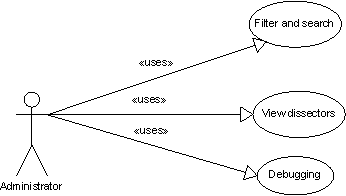
\includegraphics[width=0.8\textwidth]{./planning/img/administrator}
	\caption{Use Case Diagram: Administrator\label{fig:req:ucadm}}
\end{figure}

\begin{figure}[htbp]
	\center
	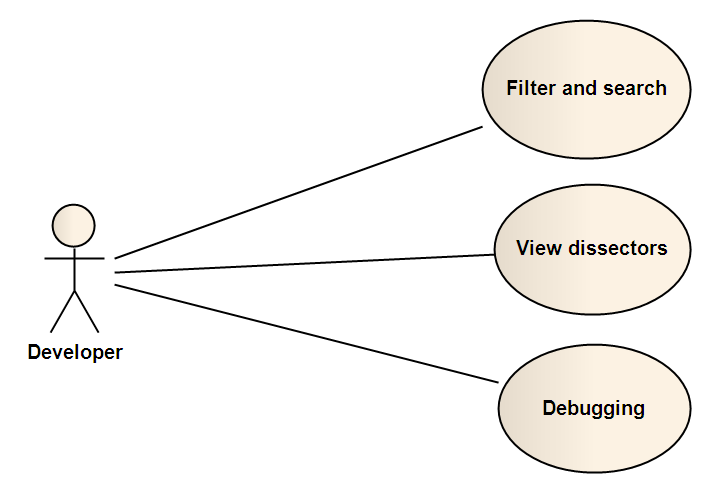
\includegraphics[width=0.8\textwidth]{./planning/img/developer}
	\caption{Use Case Diagram: Developer\label{fig:req:ucdev}}
\end{figure}

%Removed for pre-delivery
%\subsection{Textual Use Cases}
%-----------------------------
%TODO!!!

